\section{はじめに}

本書は初めてSCALEモデルを利用するユーザー向けに,SCALE-LESモデルのインストールから実行までを解説したユーザーズガイドです.
本書中のシェルコマンド等はbash を想定して記述しています.異なる環境下では適宜読み替えて対応してください.
本書中の不明点やお気づきの点がございましたら,
SCALE user's メーリングリスト \verb|scale-user@riken.jp|までご連絡ください.

\subsection{SCALEの特徴}
SCALEとは計算機を用いて気象・気候科学の問題にアプローチする際に,事前処理から数値モデル計算,解析に至るまですべてを網羅する計算ライブラリの開発を目指したソフトウェアであり,下記に挙げる特徴を持つ.
\begin{itemize}
\item SCALEは, ''Scalable Computing for Advanced Library and Environment''の略である.
\item SCALEは,フリーソフトウェアである.「BSD-2ライセンス」においてフリーソフトウェアとして提供されており,商用、非商用に関わらず自由な利用・改変が可能なソフトウェアである.
\item SCALEには,SCALE-LESモデル,SCALE-GMといった組み上げ済みの数値モデルが含まれている.
\item SCALEには,次節に示すさまざまなコンポーネントが導入されており,必要に応じて取り替えることが可能性である.
\end{itemize}

本書では,SCALEのさまざまな要素のうち,SCALE-LESモデルのインストールと実行方法について解説する.

\subsection{SCALE-LESモデルの構成}
現在,SCALE-LESモデルとして組み込まれているコンポーネントは下記のものである.
詳細なモデル構成や差分化手法については,\cite{scale_2015}を参照されたい.\\

\noindent{\bf フレームワーク関係}

\begin{itemize}
 \item Cartesian グリッドシステム(Arakawa C-grid)
 \item Cartesian ベースMPI通信
 \item Map-projection \& Map-factors
 \item Nesting システム(1-way, offline, and online)
 \item Bulk Job システム
 \item gtoolベースnetcdf4ファイル I/O
 \item JMA-GSM, JMA-MSM, WRF-ARW,NICAM向け外部データ読み込み
\end{itemize}

{\bf 力学コア関係}

\begin{itemize}
 \item 方程式系: 3次元完全圧縮流体方程式
 \item 数値解法: HE-VE,  HE-VI,HI-VIスキームから選択可能
 \item 空間差分: 4次中央差分
 \item 時間差分: 3次ルンゲクッタスキーム
 \item 非負保証: FCTスキーム
 \item 数値フィルター: 4次Hyper diffusion
 \item 地形: Terrain-followingスキーム
\end{itemize}

{\bf 物理過程}

\begin{itemize}
 \item 乱流過程: Smagorinsky typeのサブグリッドモデル, MYNN2.5境界層モデルから選択可能
 \item 雲微物理: Kessler type バルクモデル(Kessler 1969),6-class single moment バルクモデル(tomita 2006),6-class double moment バルクモデル(\cite{sn_2014}),ビン法雲モデル(\cite{suzuki_etal_2010})から選択可能
 \item 放射過程: MSTRN-X (Sekiguchi and Nakajima 2008)
 \item 地表面モデル
  \begin{itemize}
   \item 陸面モデル: バケツモデル(バルク交換係数はLouis 1994, Beljours)
   \item 海洋モデル:(スラブモデル)
   \item 都市モデル: 単層キャノピーモデル(\cite{kusaka_2001})
  \end{itemize}
\end{itemize}

上記に加えて,SCALE-LESモデル本体のドライバー,現実事例の計算に必要な地形や土地利用データを作成するツール,
理想実験の初期値・境界値,もしくは外部モデルから初期値・境界値を作成するツールが提供されている.

次節でSCALEライブラリの思想とモデルの関係について説明するが、SCALE-LESモデルの実行とは直接関係ないため,
必要なければ読み飛ばしても構わない.


\subsection{SCALEのライブラリとモデル}
SCALEは、理化学研究所 計算科学研究機構(AICS)を中心に開発が進められている気象・気候科学向けのライブラリである.
Figure \ref{fig:scale}に示されるように,このライブラリは次世代のスーパーコンピュータから汎用計算機に至るまで広く
用いられる事を念頭において開発されており,気候・気象科学を専門とする科学者と計算機科学を専門とする科学者が共同で開発を行っている.
そのため,スーパーコンピュータ「京」やFujitsu FX10等のスーパーコンピュータ上でも,ユーザーがチューニングすることなく高い計算効率で実行可能なようになっている.

SCALEライブラリは京コンピュータをはじめとする並列計算機に対してチューニングされたモデルコンポーネントや
解析システム、およびテストセットや知見といった開発環境を提供することによって、これらの問題を解決することを目的としている.

SCALEライブラリを使用して構築された数値モデルの1例がSCALE-LESモデルである(Fig. \ref{fig:scale-les})。
格子系や力学コア,物理過程といったモデル構築に必要な基本的なコンポーネントはSCALEライブラリが提供するため、
SCALE-LESモデルとして新たに用意されたのは、これらのコンポーネントをmanageするためのモデルドライバーや変数セットである。
SCALEライブラリをインストールしておくことで、SCALE-LESモデルと同様な方法によってユーザーは新たなモデル作ることができる。

\begin{figure}[t]
\begin{center}
  
\includegraphics[width=0.6\hsize]{./figure/library.eps}\\
  \caption{SCALEライブラリのねらい}
  \label{fig:scale}
\end{center}
\end{figure}

\begin{figure}[t]
\begin{center}
  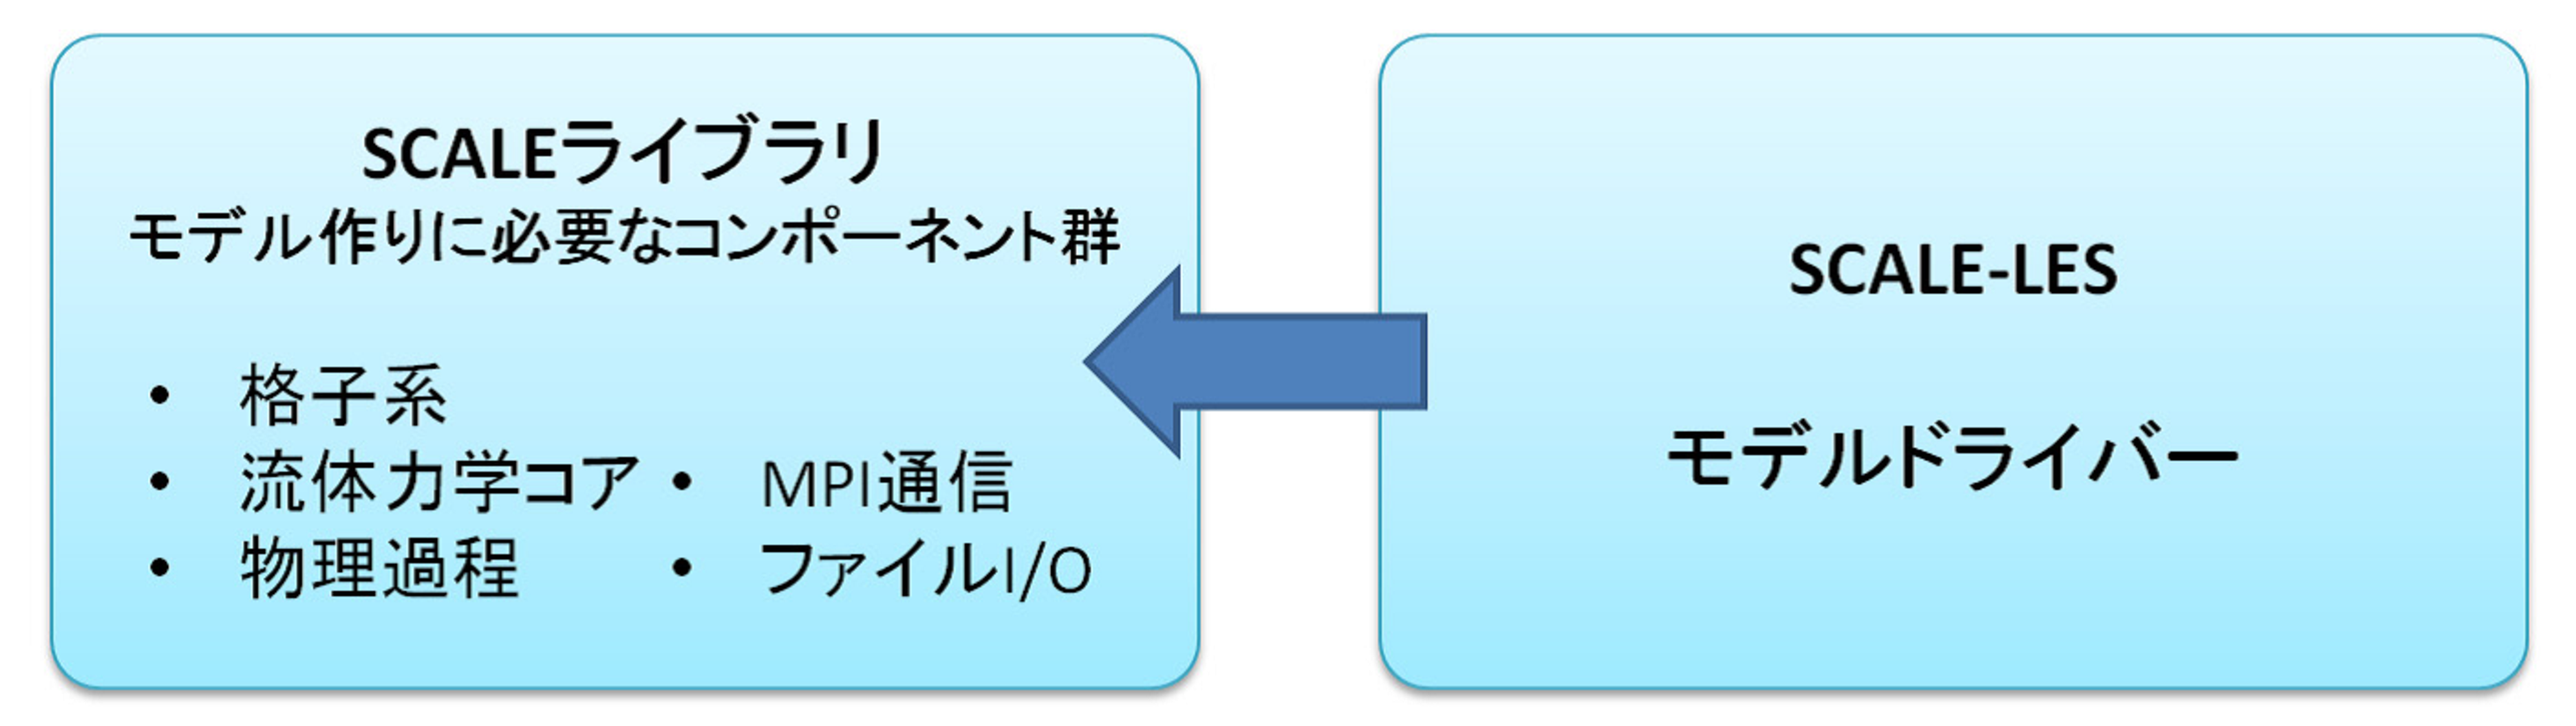
\includegraphics[width=0.9\hsize]{./figure/scale_and_scale-les.eps}\\
  \caption{SCALEライブラリとSCALE-LESモデルの関係}
  \label{fig:scale-les}
\end{center}
\end{figure}
